We can apply \gpmem\ for regression in a hierarchical Bayesian setting
(Fig. \ref{fig:neal_tutorial}).  
%%%%%%%%%%%%%%%%%%%%%%%%%%%%%%%%%%%%%%%%%%%%%%%%%%%%%%%%%%%%
\begin{figure}
\renewcommand{\arraystretch}{0.1}% Tighter
\centering \footnotesize
\begin{tikzpicture}
\node[] (start) {};
\node[left=1cm of start] (sfsigma) {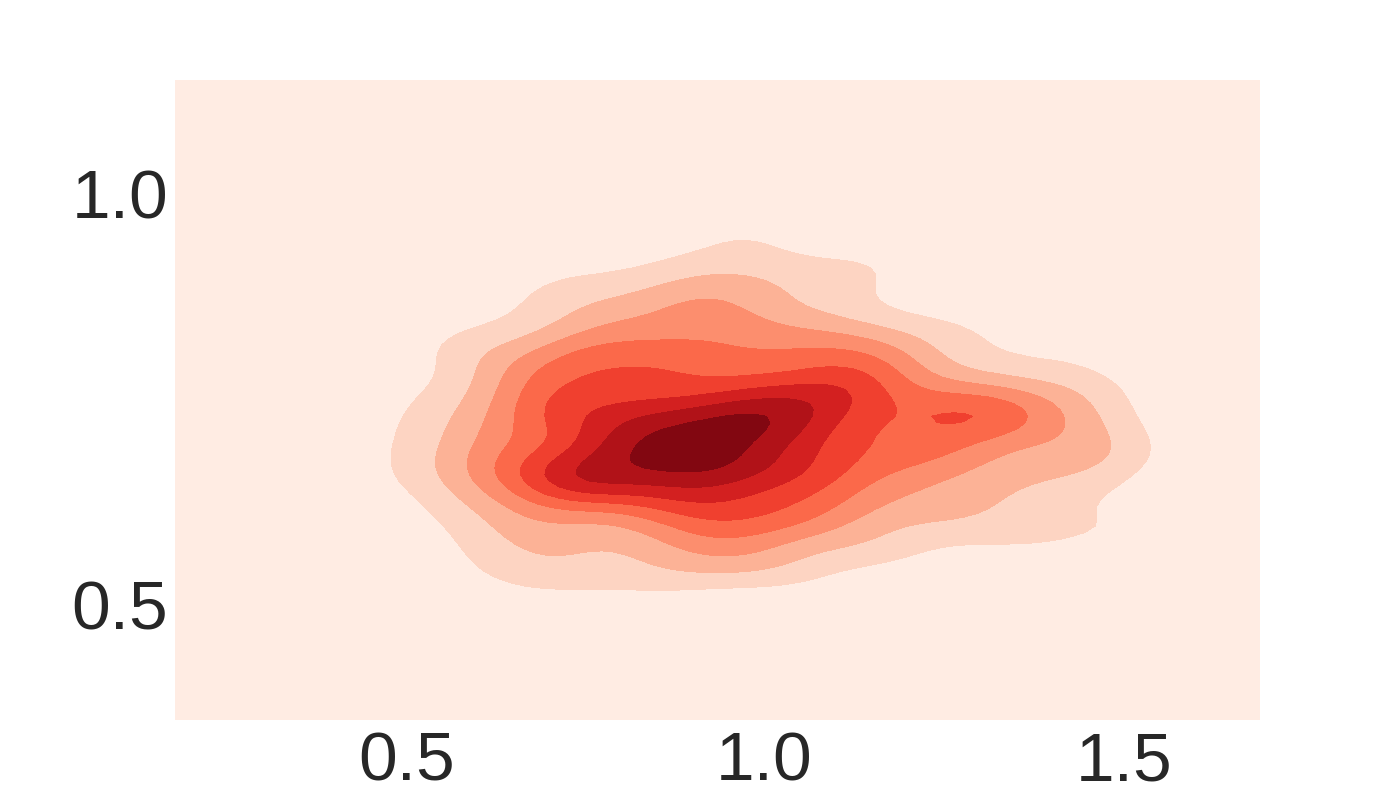
\includegraphics[height=2cm]{figs/hypers_sf_sigma.png}};
\node[right=1cm of start] (sfell) {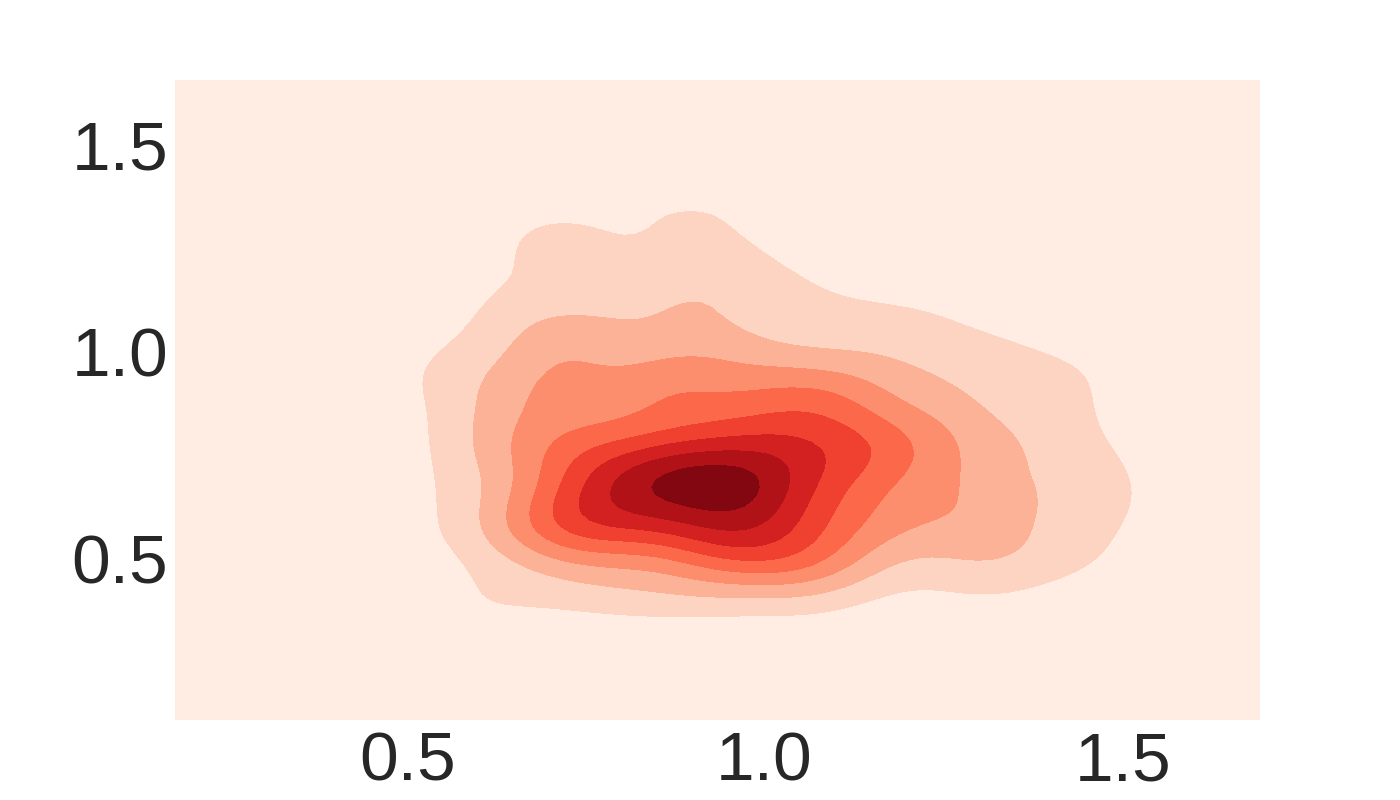
\includegraphics[height=2cm]{figs/hypers_sf_ell.png}};
\node[above=1cm of start] (hyper) {Hyper-Parameters for the Kernel:};
\node[left=0.cm of sfsigma] (ell) {$\ell$};
\node[below=0.cm of sfsigma] (sf1) {$sf$};
\node[left=0.cm of sfell] (sigma) {$\sigma$};
\node[below=0.cm of sfell] (sf2) {$sf$};
\end{tikzpicture}
\begin{tabular}{ll} \hline
\multicolumn{2}{}{}
  \begin{minipage}{4cm}
 \footnotesize\begin{lstlisting}
 // Data and look-up function
 define data = array(array(-1.87,0.13),..., array(1.67,0.81)) 
 assume f_look_up = proc(index) {lookup( data, index)}
\end{lstlisting}
\end{minipage}\\
\hline
\multicolumn{2}{}{}
  \begin{minipage}{4cm}
 \footnotesize\begin{lstlisting} 
 assume sf = tag(quote(hyper), 0, gamma(alpha_sf, beta_sf)))
 assume l = tag(quote(hyper), 1, gamma(alpha_l, beta_l)))
 assume sigma = tag(quote(hyper), 2, uniform_continuous(0, 2)) 
\end{lstlisting}
\end{minipage}
  \\
\hline
\footnotesize\begin{lstlisting}[ belowcaptionskip=0.1\baselineskip,mathescape,escapechar=\#]
// The covariance function
assume se = make_squaredexp(sf, l)
assume wn = make_whitenoise(sigma)
assume composite_covariance = add_funcs(se, wn)#\vspace{1mm}#
// Create a prober and emulator using gpmem
assume (f_compute, f_emu)
      = gpmem(f_look_up, composite_covariance)#\vspace{1mm}#
sample f_emu( array( -2, $\cdots$, 2)) 
\end{lstlisting}
 &  \raisebox{-0.5\height}{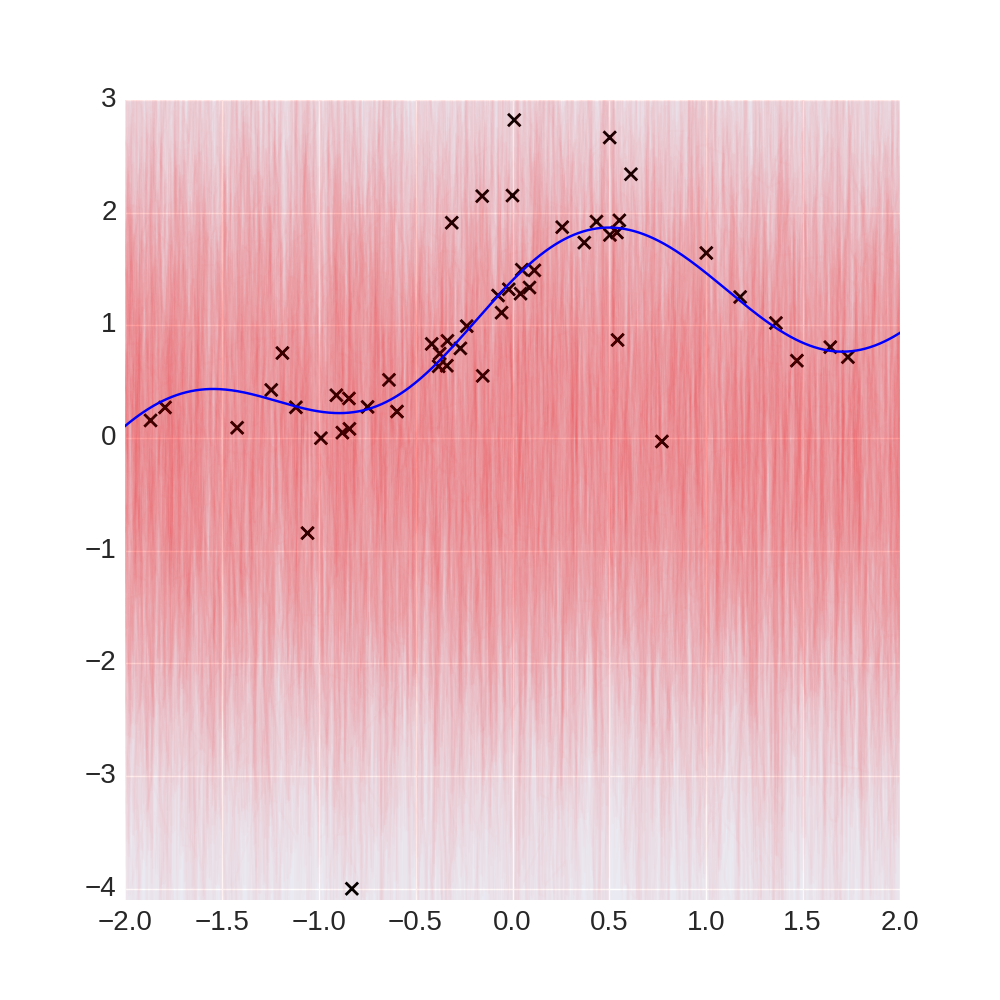
\includegraphics[height=3.4cm]{figs/neal_example_before_observation.png}}  \\ \hline
% line 3 

\footnotesize\begin{lstlisting}[aboveskip=-0.8 \baselineskip,mathescape,escapechar=\#]
// Observe all data points
for n ... N
    observe f_emu(first(lookup(data,n))) 
                = second(lookup(data,n))
// Or: probe all data points
for n ... N
    predict f_compute(first(lookup(data,n)))#\vspace{1mm}#
sample f_emu( array( -2, $\cdots$, 2)) 
\end{lstlisting}
 &  \raisebox{-0.5\height}{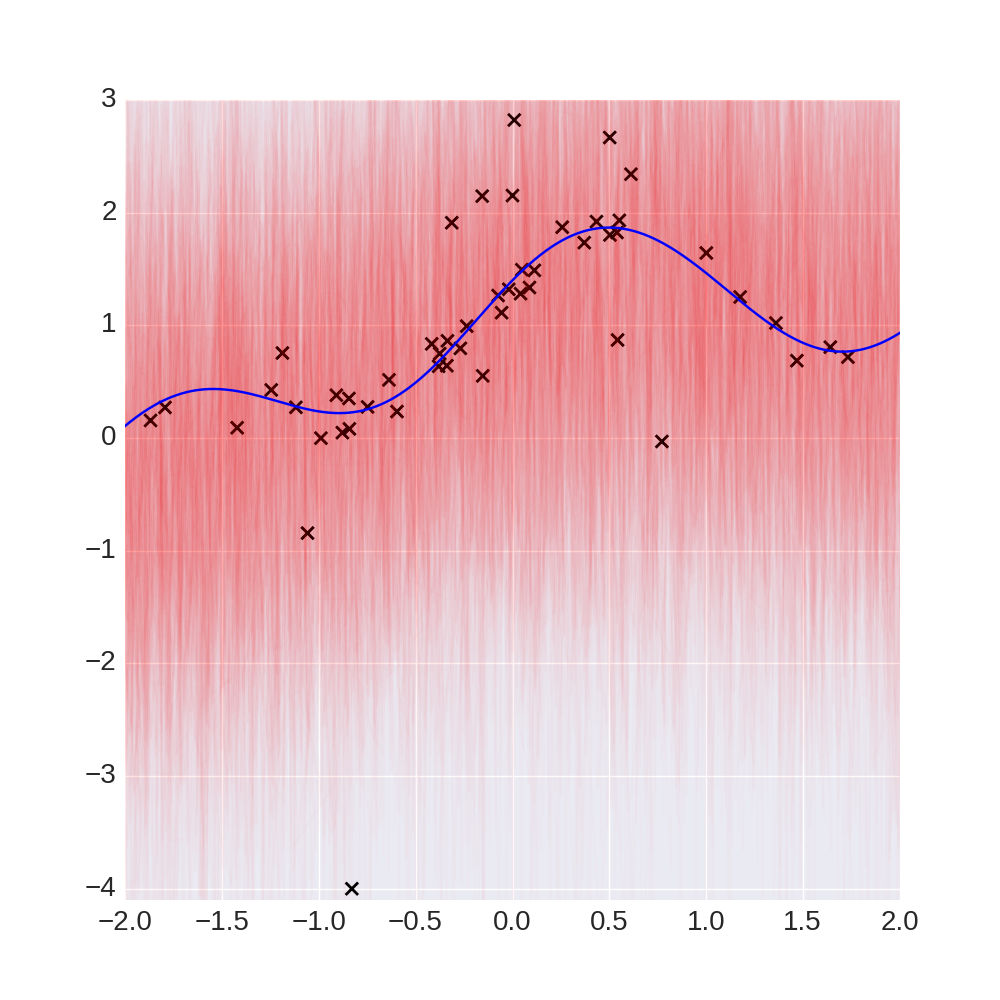
\includegraphics[height=3.4cm]{figs/neal_example_after_observation.png}}  \\ \hline
\footnotesize\begin{lstlisting}[mathescape,escapechar=\#]
// Metropolis-Hastings
infer repeat( 100, do(
                   mh( quote(hyperhyper), one, 2),
		   mh( quote(hyper),      one, 1)))#\vspace{1mm}#
sample f_emu( array( -2, $\cdots$, 2))   
\end{lstlisting}
 &   \raisebox{-0.5\height}{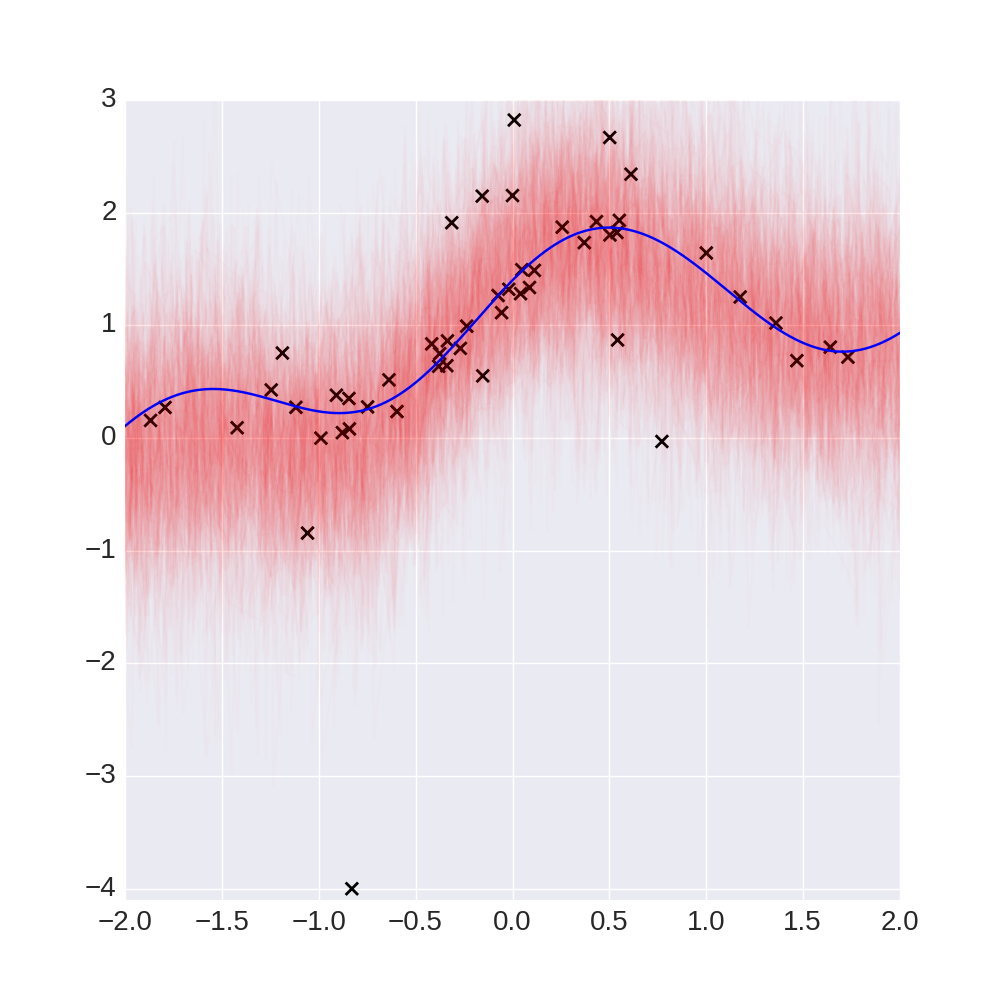
\includegraphics[height=3.4cm]{figs/neal_Bayesian.png}} \\ \hline
\footnotesize\begin{lstlisting}[mathescape,escapechar=\#]
// Optimization 
infer map( quote(hyper), all,0.01, 15)

sample f_emu( array( -2, $\cdots$, 2)) 
\end{lstlisting}
 &   \raisebox{-0.5\height}{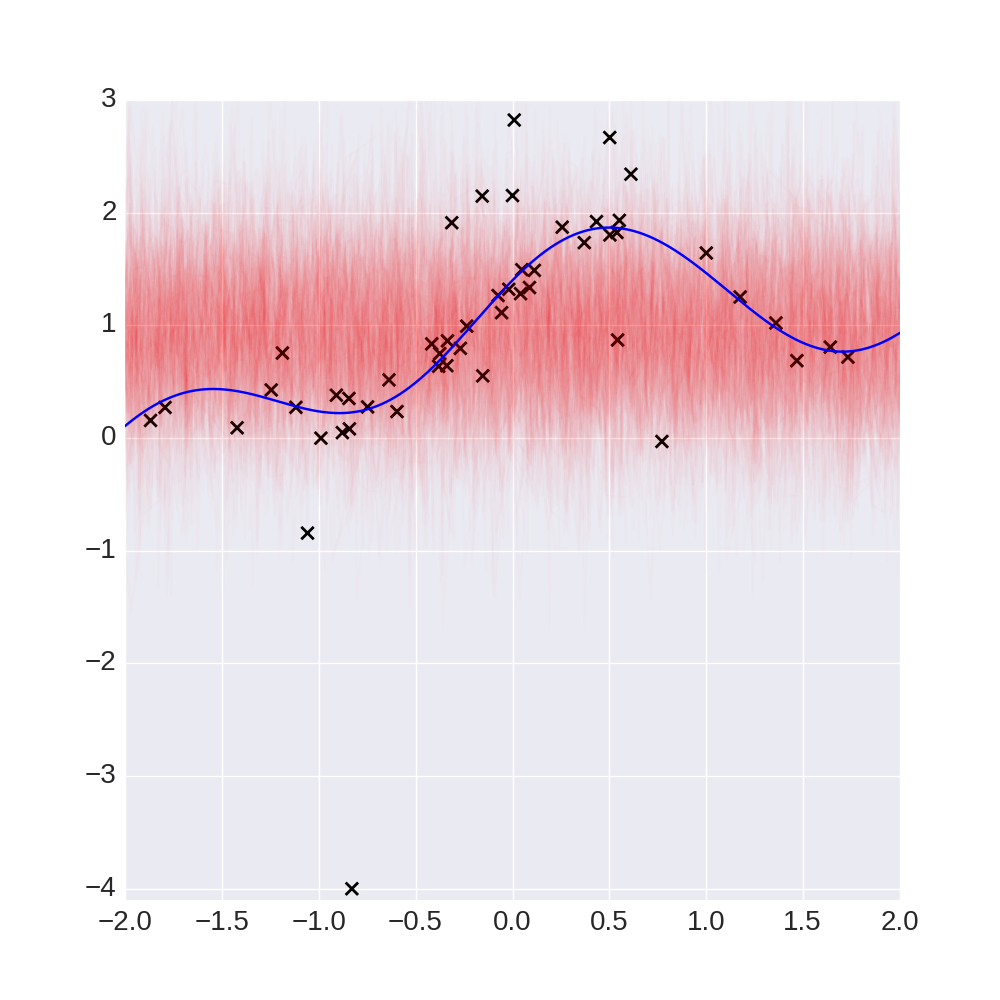
\includegraphics[height=3.4cm]{figs/neal_example_map_inference_alpha0p01_iter15.png}} \\ \hline
 
 \end{tabular}
\captionsetup{aboveskip=-7pt}
\caption{\footnotesize Regression with outliers and hierarchical prior
structure.}
\label{fig:neal_tutorial}
\end{figure}
%%%%%%%%%%%%%%%%%%%%%%%%%%%%%%%%%%%%%%%%%%%%%%%%%%%%%%%%%%%%
In a Bayesian treatment of  hyper-parameter learning for \ac{GP}s,
we can write the posterior probability of the hyper-parameters of a GP  (Fig.
\ref{fig:neal_tutorial}, (a)) given covariance function $\Krv=k$ as:
%%%%%%%%%%%%%%%%%%%%%%%%%%%%%%%%%%%%%%%%%%%%%%%%%%%%%%%%%%%%
\begin{equation}
\label{eq:hyperProbability}
P(\thetabf=\{sf,\ell,\sigma\} \mid \mathbf{D},\Krv ) = \frac{P(\mathbf{D} \mid
\thetabf, \Krv)P(\thetabf \mid \Krv) }{P(\mathbf{D} \mid
\Krv)}
\end{equation}
%%%%%%%%%%%%%%%%%%%%%%%%%%%%%%%%%%%%%%%%%%%%%%%%%%%%%%%%%%%%
where $\mathbf{D} = \{\xbf, \ybf\}$ is a training data set and $\Krv$ is treated
as a random variable over covariance functions.

We demonstrate \gpmem's application to regression using an example
taken from a paper on the treatment of outliers with hierarchical
Bayesian hyper-priors for \ac{GP}s~\citep{neal1997monte}:
%%%%%%%%%%%%%%%%%%%%%%%%%%%%%%%%%%%%%%%%%%%%%%%%%%%%%%%%%%%%
\begin{equation}
f_\text{true}(x) =  0.3 + 0.4 x + 0.5 \sin(2.7x) + \frac{1.1}{(1+ x^2)} + \eta
\;\;\; with\;\;\eta \sim \mathcal{N}(0,\sigmanoise). \label{eq:f_true}
\end{equation}
%%%%%%%%%%%%%%%%%%%%%%%%%%%%%%%%%%%%%%%%%%%%%%%%%%%%%%%%%%%%
We emphasize that \gpmem\ can be used with externally collected
data sets whose generating process may not be available at all,
by coding the ``true function'' argument to \gpmem\ as a lookup
in a fixed data set (Fig. \ref{fig:neal_tutorial} (b)).
That data was synthesized offline by applying the $f_\text{true}$ of (\ref{eq:f_true})
to a fixed set of inputs, with outliers given by setting $\sigmanoise = 1$ in 5\% of
the cases (the remaining 95\% ``inliers'' have $\sigmanoise = 0.1$).

We set $\Krv = k^{\text{se}+\text{wn}}$ and parameterize it with $\bm{\theta}=\{sf,\ell,\sigma\}$.
For these hyper-parameters, Neal's work suggests a hierarchical system for
hyper-parameterization.
Here, we draw hyper-parameters from $\Gamma$ distributions:
%%%%%%%%%%%%%%%%%%%%%%%%%%%%%%%%%%%%%%%%%%%%%%%%%%%%%%%%%%%%
\begin{equation}
\label{eq:hyper-ell}
\ell \sim \Gamma(\alpha_1,\beta_1),\;\sigma \sim \Gamma(\alpha_2,\beta_2)
\end{equation} 
%%%%%%%%%%%%%%%%%%%%%%%%%%%%%%%%%%%%%%%%%%%%%%%%%%%%%%%%%%%%
and in turn sample the $\alpha$ and $\beta$ from $\Gamma$ distributions as well:
%%%%%%%%%%%%%%%%%%%%%%%%%%%%%%%%%%%%%%%%%%%%%%%%%%%%%%%%%%%%
\begin{equation}
\label{eq:hyper-alpha}
\alpha_1 \sim \Gamma(\alpha^1_{\alpha},\beta^1_{ \alpha } ),\; \alpha_2 \sim \Gamma(\alpha^2_{\alpha},\beta^2_{\alpha}),\cdots
\end{equation}
%%%%%%%%%%%%%%%%%%%%%%%%%%%%%%%%%%%%%%%%%%%%%%%%%%%%%%%%%%%%
We model this in Venture as illustrated in Fig. \ref{fig:neal_tutorial} (c),
using the built-in \ac{SP} $\texttt{gamma}$. 

In Fig. \ref{fig:neal_tutorial}, panel (d), we see that $k^{\text{se}+\text{wn}}$
is defined as a composite covariance function. It is the sum ($\texttt{add\_funcs}$) of
a squared exponential kernel ($\texttt{make\_squaredexp}$) and a white noise
($\kwn$, Appendix A)
kernel which is implemented with $\texttt{make\_whitenoise}$\footnote{Note
that in Neal's work \citeyearpar{neal1997monte} the sum of an SE
plus a constant kernel is used. We use a WN kernel for illustrative purposes
instead.}. 
We then initialize \gpmem\ feeding it with $\texttt{composite\_covariance}$ and the data
look-up function $\texttt{f\_look\_up}$. 
We sample from the prior $\ystar$ with random parameters $\texttt{sf,l}$ and $\texttt{sigma}$ and 
without any observations available (Fig. \ref{fig:neal_tutorial}, panel (e)).
We depict those samples on the right (red), alongside the true function that generated the data (blue) and
the data points we have available in the data set (black).

We can incorporate observations using both \texttt{observe} and \texttt{predict} (Fig. \ref{fig:neal_tutorial} (f)).
When we subsequently sample $\yprime$ from the emulator with
$\mathcal{N}(\mupost,\Kpost)$, we can see that the \ac{GP} posterior incorporates knowledge 
about the $\texttt{data}$. Yet, the hyper-parameters $\texttt{sf,l}$ and $\texttt{sigma}$ are still
random, so the emulator does not capture the true underlying dynamics
($f_\text{true}$) of the \texttt{data} correctly. 

Next, we demonstrate how we can capture these underlying dynamics within only
100  nested \ac{MH} steps on the hyper-parameters to get a good approximation
for their posterior $\yprime$ (Fig. \ref{fig:neal_tutorial} (g)).
We say nested because we first take two sweeps in the scope
$\texttt{hyperhyper}$ which characterizes (\ref{eq:hyper-alpha}) and then one
sweep on the scope $\texttt{hyper}$ which characterizes (\ref{eq:hyper-ell}).
This is repeated 100 times using $\texttt{repeat( 100, do(}\cdots\;$.
Note that Neal devises an additional noise model and performs a large number of Hybrid-Monte Carlo and Gibbs steps to achieve this, whereas inference in Venture with \gpmem\ is merely one line of code. 

Finally, we can change our inference strategy altogether. If we decide that instead of
following a Bayesian sampling approach, we would like to perform empirical optimization,
we do this by only changing one line of code, deploying $\texttt{gradient-ascent}$ instead
of $\texttt{mh}$ (Fig. \ref{fig:neal_tutorial} (h)). 

